\documentclass[tikz,border=10pt]{standalone}
\begin{document}
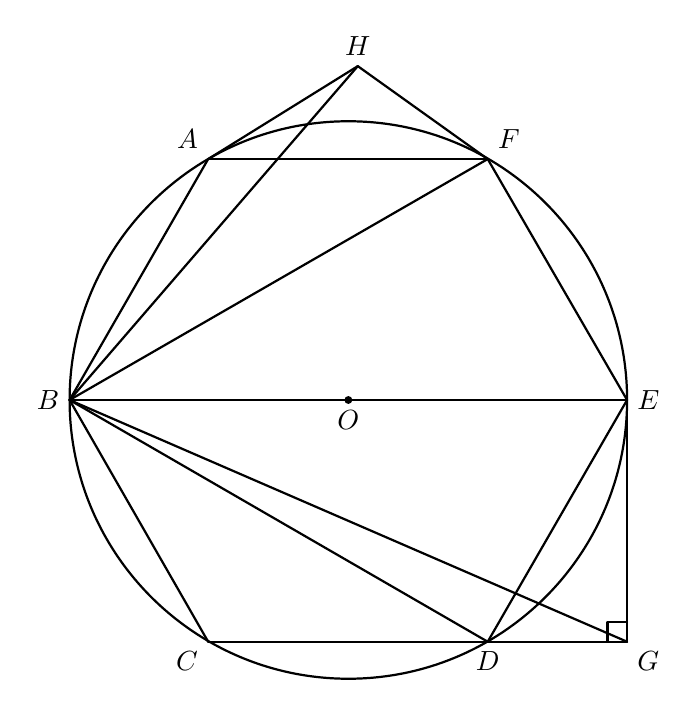
\begin{tikzpicture}[scale=1, line cap=round, line join=round, thick]
  % Points
  \coordinate (O) at (0,0);
  \coordinate (B) at (-3.54,0);
  \coordinate (E) at (3.54,0);
  \coordinate (H) at (0.12,4.24);
  \coordinate (A) at (-1.78,3.06);
  \coordinate (F) at (1.77,3.06);
  \coordinate (C) at (-1.78,-3.07);
  \coordinate (D) at (1.77,-3.07);
  \coordinate (G) at (3.54,-3.07);

  % Circle
  \draw (O) circle (3.54);

  % Edges
  \draw (H) -- (A);
  \draw (H) -- (F);
  \draw (H) -- (B);
  \draw (A) -- (F);
  \draw (B) -- (A);
  \draw (B) -- (F);
  \draw (B) -- (E);
  \draw (B) -- (C);
  \draw (B) -- (D);
  \draw (B) -- (G);
  \draw (F) -- (E);
  \draw (E) -- (D);
  \draw (C) -- (D) -- (G);
  \draw (E) -- (G);

  % Right angle mark at G
  \draw (3.54,-2.82) -- (3.29,-2.82) -- (3.29,-3.07);

  % Dot at O
  \fill (O) circle (0.05);

  % Labels
  \node[above] at (H) {$H$};
  \node[above left] at (A) {$A$};
  \node[above right] at (F) {$F$};
  \node[left] at (B) {$B$};
  \node[right] at (E) {$E$};
  \node[below] at (O) {$O$};
  \node[below left] at (C) {$C$};
  \node[below] at (D) {$D$};
  \node[below right] at (G) {$G$};
\end{tikzpicture}
\end{document}
